\documentclass[tikz,border=2pt]{standalone}
\usepackage{amsmath,amssymb}
\usepackage{tikz}
\usetikzlibrary{arrows.meta}

\begin{document}
% The image f(C) collects the outputs of a set C; the preimage f^{-1}(D) collects every input
% whose output lands in D (it may be empty or contain several points per element of D).
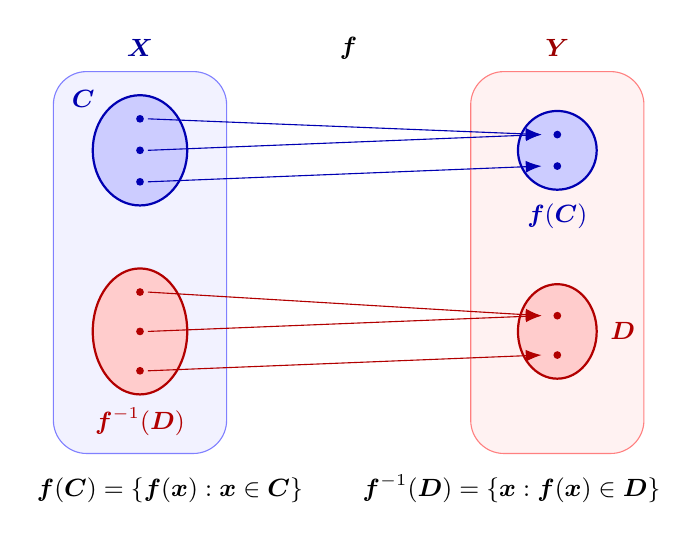
\begin{tikzpicture}[every node/.style={font=\small}, >={Latex[length=2mm]}]
	\draw[rounded corners=12pt, fill=blue!5, draw=blue!50] (-1.1,-2.65) rectangle (1.1,2.2);
	\draw[rounded corners=12pt, fill=red!5, draw=red!50] (4.2,-2.65) rectangle (6.4,2.2);
	\node[blue!60!black] at (0,2.5) {$\boldsymbol{X}$}; \node[red!60!black] at (5.3,2.5) {$\boldsymbol{Y}$};
	% C and its image
	\draw[blue!70!black, thick, fill=blue!20] (0,1.2) ellipse (0.6 and 0.7);
	\node[blue!70!black] at (-0.72,1.85) {$\boldsymbol{C}$};
	\draw[blue!70!black, thick, fill=blue!20] (5.3,1.2) ellipse (0.5 and 0.5);
	\node[blue!70!black, anchor=north] at (5.3,0.64) {$\boldsymbol{f}(\boldsymbol{C})$};
	\foreach \y in {1.6,1.2,0.8} {\fill[blue!70!black] (0,\y) circle (1.4pt);}
	\draw[->, blue!70!black] (0.1,1.6) -- (5.1,1.4);
	\draw[->, blue!70!black] (0.1,1.2) -- (5.1,1.4);
	\draw[->, blue!70!black] (0.1,0.8) -- (5.1,1.0);
	\fill[blue!70!black] (5.3,1.4) circle (1.4pt); \fill[blue!70!black] (5.3,1.0) circle (1.4pt);
	% D and its preimage
	\draw[red!70!black, thick, fill=red!20] (5.3,-1.1) ellipse (0.5 and 0.6);
	\node[red!70!black, anchor=west] at (5.85,-1.1) {$\boldsymbol{D}$};
	\draw[red!70!black, thick, fill=red!20] (0,-1.1) ellipse (0.6 and 0.8);
	\node[red!70!black, anchor=north] at (0,-1.95) {$\boldsymbol{f}^{-1}(\boldsymbol{D})$};
	\foreach \y in {-0.6,-1.1,-1.6} {\fill[red!70!black] (0,\y) circle (1.4pt);}
	\fill[red!70!black] (5.3,-0.9) circle (1.4pt); \fill[red!70!black] (5.3,-1.4) circle (1.4pt);
	\draw[->, red!70!black] (0.1,-0.6) -- (5.1,-0.9);
	\draw[->, red!70!black] (0.1,-1.1) -- (5.1,-0.9);
	\draw[->, red!70!black] (0.1,-1.6) -- (5.1,-1.4);
	\node[anchor=north, align=center] at (2.65,-2.8) {$\boldsymbol{f}(\boldsymbol{C})=\{\boldsymbol{f}(\boldsymbol{x}):\boldsymbol{x}\in\boldsymbol{C}\}$ \qquad $\boldsymbol{f}^{-1}(\boldsymbol{D})=\{\boldsymbol{x}:\boldsymbol{f}(\boldsymbol{x})\in\boldsymbol{D}\}$};
	\node at (2.65,2.5) {$\boldsymbol{f}$};
\end{tikzpicture}
\end{document}
